\documentclass[aspectratio=169]{../latex_main/tntbeamer}  % you can pass all options of the beamer class, e.g., 'handout' or 'aspectratio=43'
\usepackage{dsfont}
\usepackage{bm}
\usepackage[english]{babel}
\usepackage[T1]{fontenc}
%\usepackage[utf8]{inputenc}
\usepackage{graphicx}
\graphicspath{ {./figures/} }
\usepackage{algorithm}
\usepackage[ruled,vlined,algo2e,linesnumbered]{algorithm2e}
\usepackage{hyperref}
\usepackage{booktabs}
\usepackage{mathtools}

\usepackage{amsmath,amssymb}

\DeclareMathOperator*{\argmax}{arg\,max}
\DeclareMathOperator*{\argmin}{arg\,min}

\usepackage{amsbsy}
\newcommand{\vect}[1]{\bm{#1}}
%\newcommand{\vect}[1]{\boldsymbol{#1}}

\usepackage{pgfplots}
\pgfplotsset{compat=1.16}
\usepackage{tikz}
\usetikzlibrary{trees} 
\usetikzlibrary{shapes.geometric}
\usetikzlibrary{positioning,shapes,shadows,arrows,calc,mindmap}
\usetikzlibrary{positioning,fadings,through}
\usetikzlibrary{decorations.pathreplacing}
\usetikzlibrary{intersections}
\pgfdeclarelayer{background}
\pgfdeclarelayer{foreground}
\pgfsetlayers{background,main,foreground}
\tikzstyle{activity}=[rectangle, draw=black, rounded corners, text centered, text width=8em]
\tikzstyle{data}=[rectangle, draw=black, text centered, text width=8em]
\tikzstyle{myarrow}=[->, thick, draw=black]

% Define the layers to draw the diagram
\pgfdeclarelayer{background}
\pgfdeclarelayer{foreground}
\pgfsetlayers{background,main,foreground}

% Requires XeLaTeX or LuaLaTeX
%\usepackage{unicode-math}

\usepackage{fontspec}
%\setsansfont{Arial}
\setsansfont{RotisSansSerifStd}[ 
Path=../latex_main/fonts/,
Extension = .otf,
UprightFont = *-Regular,  % or *-Light
BoldFont = *-ExtraBold,  % or *-Bold
ItalicFont = *-Italic
]
\setmonofont{Cascadia Mono}[
Scale=0.8
]

% scale factor adapted; mathrm font added (Benjamin Spitschan @TNT, 2021-06-01)
%\setmathfont[Scale=1.05]{Libertinus Math}
%\setmathrm[Scale=1.05]{Libertinus Math}

% other available math fonts are (not exhaustive)
% Latin Modern Math
% XITS Math
% Libertinus Math
% Asana Math
% Fira Math
% TeX Gyre Pagella Math
% TeX Gyre Bonum Math
% TeX Gyre Schola Math
% TeX Gyre Termes Math

% Literature References
\newcommand{\lit}[2]{\href{#2}{\footnotesize\color{black!60}[#1]}}

%%% Beamer Customization
%----------------------------------------------------------------------
% (Don't) Show sections in frame header. Options: 'sections', 'sections light', empty
\setbeamertemplate{headline}{empty}

% Add header logo for normal frames
\setheaderimage{
	% 
\includegraphics[height=\logoheight]{figures/TNT_darkv4.pdf}
	
\includegraphics[height=\logoheight]{../latex_main/figures/luh_logo_rgb_0_80_155.pdf}
	% 
\includegraphics[height=\logoheight]{figures/logo_tntluh.pdf}
}

% Header logo for title page
\settitleheaderimage{
	% 
\includegraphics[height=\logoheight]{figures/TNT_darkv4.pdf}
	
\includegraphics[height=\logoheight]{../latex_main/figures/luh_logo_rgb_0_80_155.pdf}
	% 
\includegraphics[height=\logoheight]{figures/logo_tntluh.pdf}
}

% Title page: tntdefault 
\setbeamertemplate{title page}[tntdefault]  % or luhstyle
% Add optional title image here
%\addtitlepageimagedefault{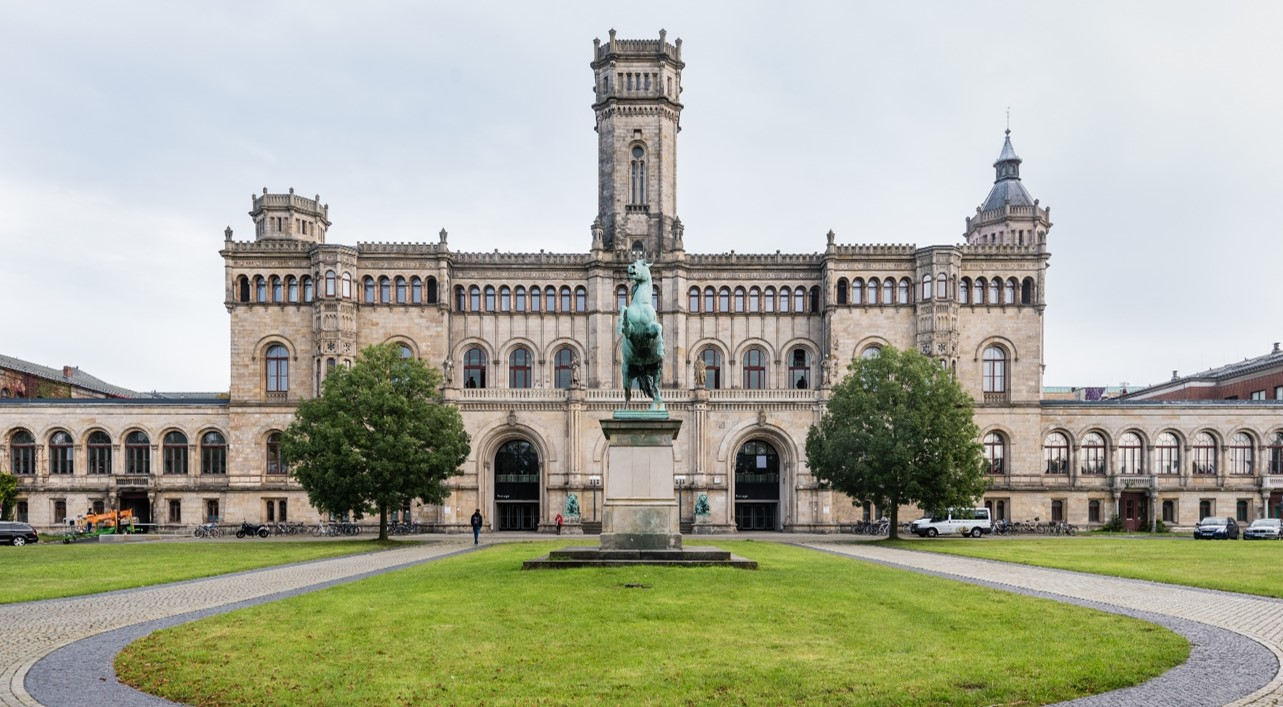
\includegraphics[width=0.65\textwidth]{figures/luh_default_presentation_title_image.jpg}}

% Title page: luhstyle
% \setbeamertemplate{title page}[luhstyle]
% % Add optional title image here
% \addtitlepageimage{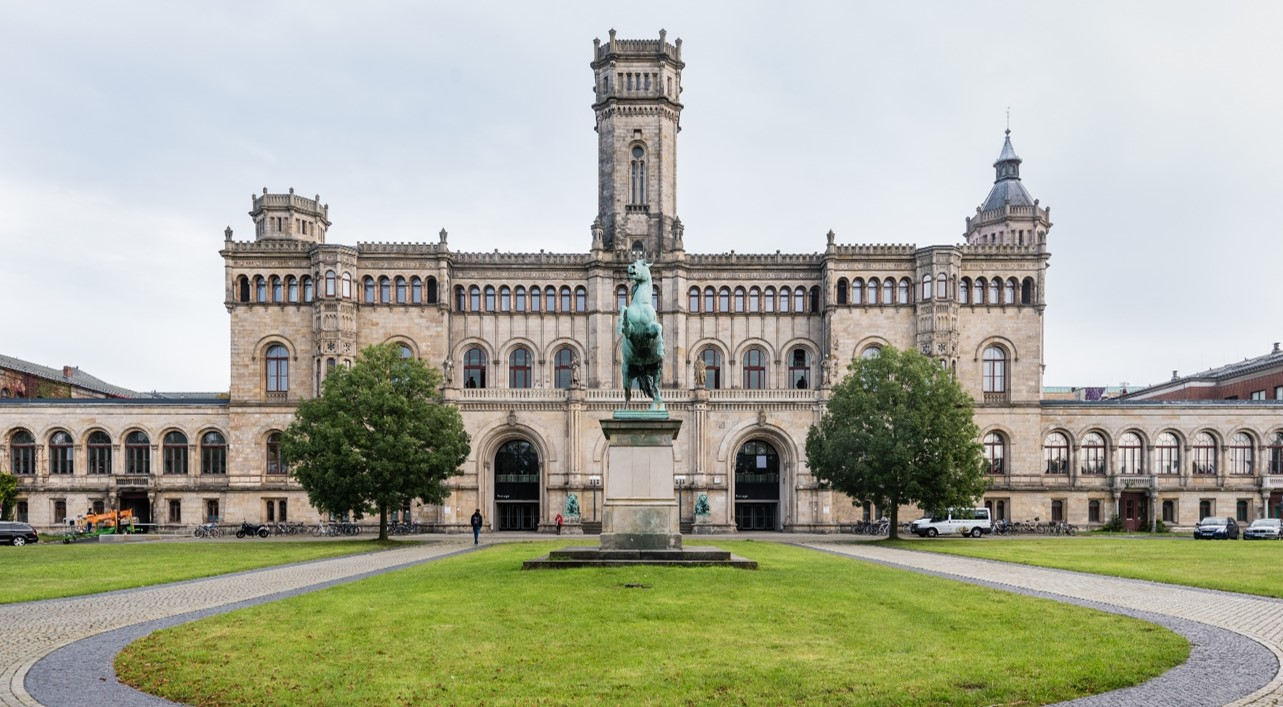
\includegraphics[width=0.75\textwidth]{figures/luh_default_presentation_title_image.jpg}}

\author[Abedjan \& Lindauer]{Ziawasch Abedjan \& Marius Lindauer\\[1em]
	
\includegraphics[height=\logoheight]{../latex_main/figures/luh_logo_rgb_0_80_155.pdf}\qquad
	
\includegraphics[height=\logoheight]{../latex_main/figures/DBIS_Kurzlogo.png}\qquad

\includegraphics[height=\logoheight]{../latex_main/figures/TNT_darkv4}\qquad

\includegraphics[height=\logoheight]{../latex_main/figures/L3S.jpg}	}
\date{Summer Term 2022; \hspace{0.5em} {
\includegraphics[height=1.5em]{../latex_main/figures/Cc-by-nc-sa_icon.svg.png}}; based on \href{https://ds100.org/fa21/}{[DS100]}
}


%%% Custom Packages
%----------------------------------------------------------------------
% Create dummy content
\usepackage{blindtext}

% Adds a frame with the current page layout. Just call \layout inside of a frame.
\usepackage{layout}


%%% Macros
%\renewcommand{\vec}[1]{\mathbf{#1}}
% \usepackage{bm}
%\let\vecb\bm

\title[Introduction]{DS: Decision Trees}
\subtitle{Decision Trees and Overfitting}

\graphicspath{ {./figure_tree/} }
%\institute{}


\begin{document}
	
	\maketitle
	\begin{frame}{Overfitting and Decision Trees}
	    With the exception of samples that have the exact same data, we can always get 100\% accuracy with decision trees. This should give us concern about possible overfitting.\\
	    \bigskip
	    Let’s see how bad things are by separating our data into train and test sets
	    \begin{itemize}
	        \item We’ll use 110 training points and 40 testing points
	        \item Performance on test set gives us an estimate of how well we generalize
	    \end{itemize}
	    \begin{figure}
	        \centering
	        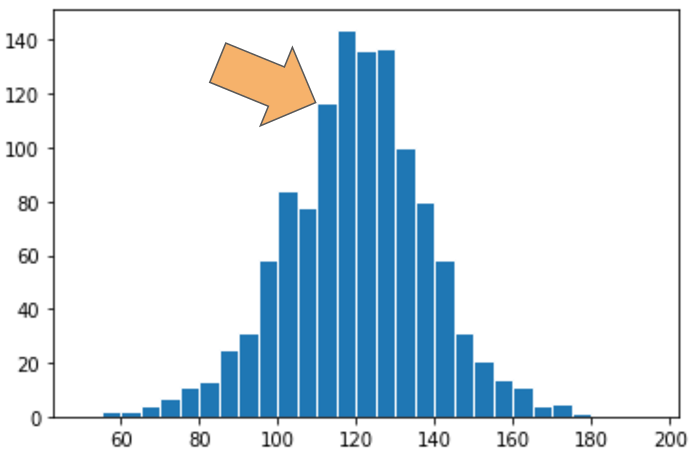
\includegraphics[scale=.4]{Bild30}
	    \end{figure}
	\end{frame}
	
	\begin{frame}{Visualizing Our New Model}
	   Comparing our model trained on 150 vs. 110 data points, we see differences in the generated model\\
	    \begin{itemize}
	        \item Naturally, both models get very high accuracy on the data that they use for training\\ (100\% for non-overlapping points)
	    \end{itemize}
	    \begin{figure}
	        \centering
	        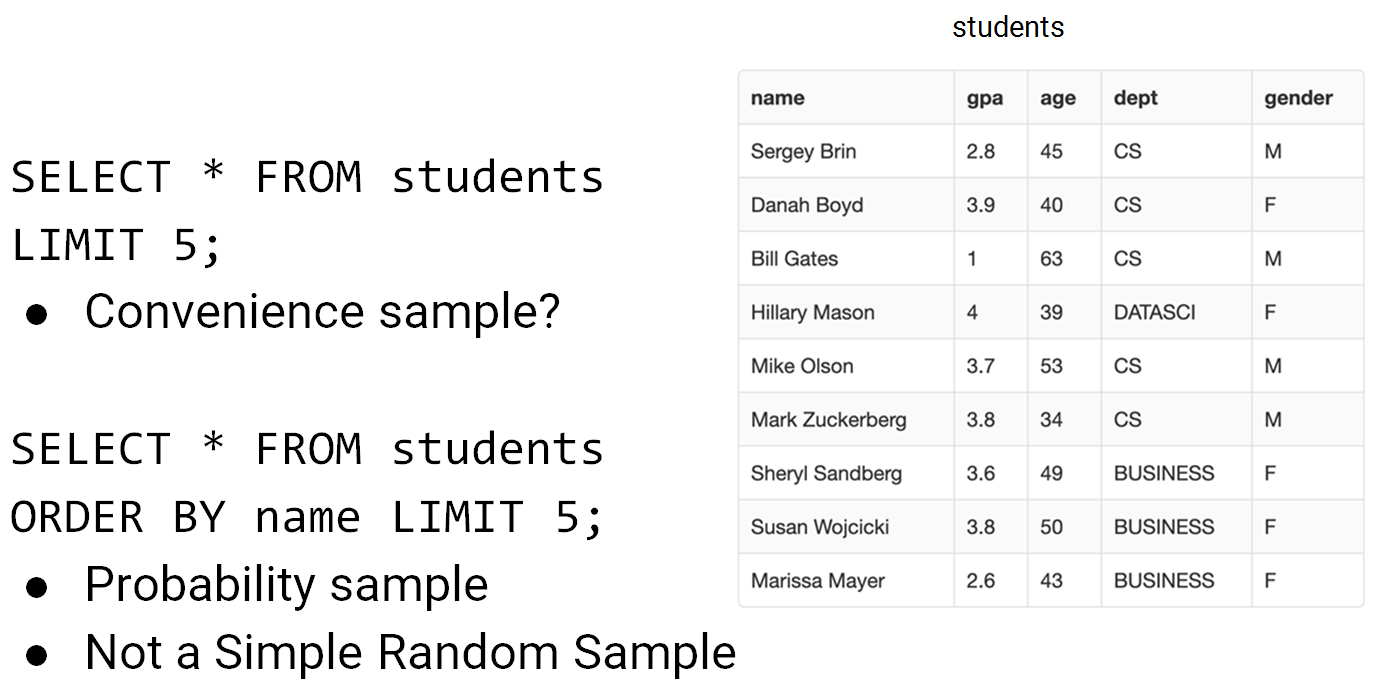
\includegraphics[scale=.4]{Bild31}
	    \end{figure}
	\end{frame}
	
	
	\begin{frame}{Performance of Our New Model on the Test Set}
	  When we look at the performance of Model 2D-110 on the test set, we see that we make some errors that aren’t just from overlapping data\\
	    \begin{itemize}
	        \item 99\% accuracy on training set (2 overlapping points). 95\% accuracy on test set
	    \end{itemize}
	    \begin{figure}
	        \centering
	        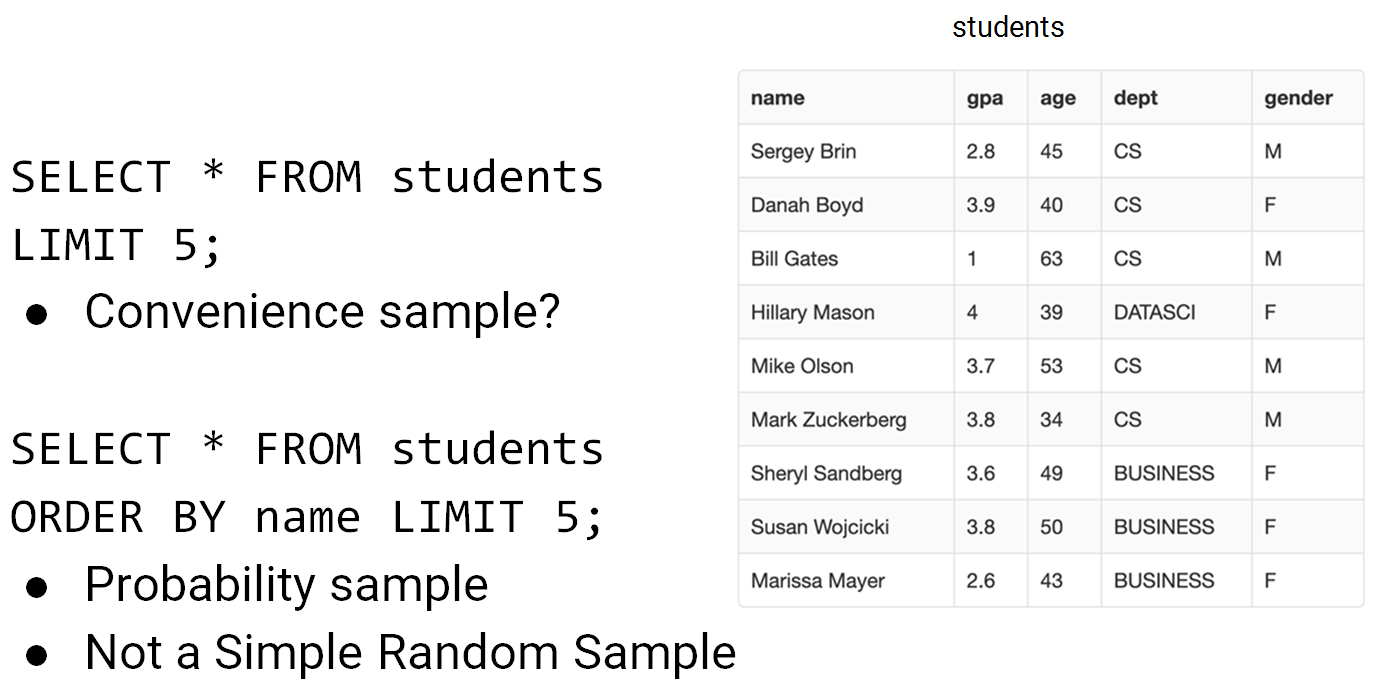
\includegraphics[scale=.4]{Bild31}
	    \end{figure}
	\end{frame}
	
	
	\begin{frame}{Multidimensional Decision Trees}
	  Naturally, we can include even more features. For example, if we want to use the petal AND sepal measurements, we simply train the decision tree on all four columns of the data\\
	  \begin{figure}
	        \centering
	        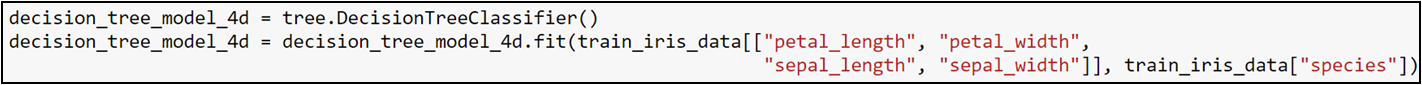
\includegraphics[scale=.6]{Bild32}
	    \end{figure}
	    The resulting model Model 4D-110 gets:
	    \begin{itemize}
	        \item 100\% accuracy on the training set (no overlapping data points)
            \item 95\% accuracy on the test set
	    \end{itemize}
	    Cannot easily visualize Model 4D-110’s decision   boundaries because the prediction space   is 4 dimensional
	\end{frame}
	
	
	\begin{frame}{Model 2D-150 vs. Model 4D-110 Tree Visualization}
	    \begin{columns}
	        \begin{column}{.5\textwidth}
	                \begin{figure}
	                    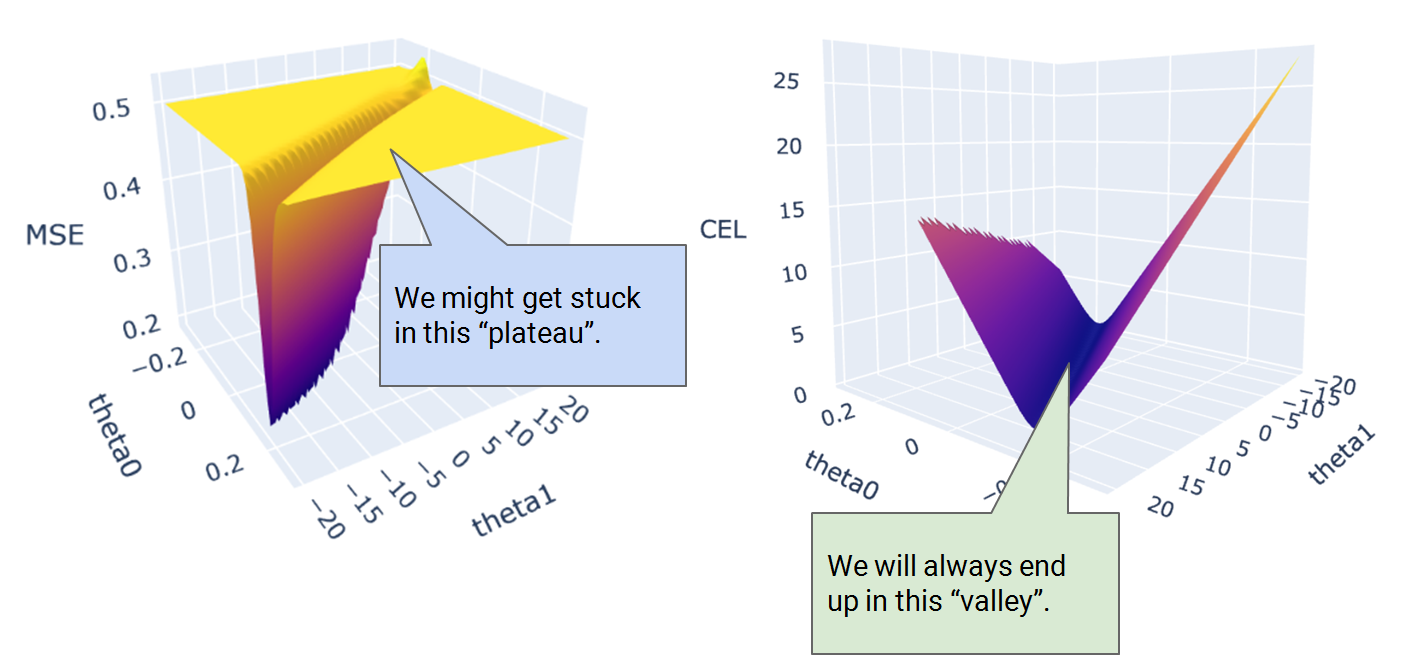
\includegraphics[scale=.53]{Bild23}
	                \end{figure}
	        \end{column}
	   
	        \begin{column}{.5\textwidth}
	                \begin{figure}
	                    
\includegraphics[scale=.33]{Bild35}
	                \end{figure}
	        \end{column}
	    \end{columns}
	    What is different about these two models?
	\end{frame}
	
	
	\begin{frame}{Model 2D-150 vs. Model 4D-110 Tree Visualization}
	    \begin{columns}
	        \begin{column}{.5\textwidth}
	                Models are quite similar:
	                \begin{itemize}
	                    \item Model 4D-110 uses only 110 samples.
	                    \item The decision rules are nearly identical, except that Model4D-110 uses the sepal\_width exactly once to resolve the case that we couldn’t resolve with petal\_length and petal\_width
	                \end{itemize}
	                Model 4D-110 seems marginally better to me, but both got only 95\% accuracy on test set. 
	                \begin{itemize}
	                    \item Need more data to know for sure
	                \end{itemize}
	        \end{column}
	   
	        \begin{column}{.5\textwidth}
	                \begin{figure}
	                    
\includegraphics[scale=.33]{Bild35}
	                \end{figure}
	        \end{column}
	    \end{columns}
	 
	\end{frame}
	
	
	
	\begin{frame}{Model 2D-150 vs. Model 4D-110 Tree Visualization}
	    \begin{columns}
	        \begin{column}{.5\textwidth}
	                Models are quite similar:
	                \begin{itemize}
	                    \item Model 4D-110 uses only 110 samples.
	                    \item The decision rules are nearly identical, except that Model4D-110 uses the sepal\_width exactly once to resolve the case that we couldn’t resolve with petal\_length and petal\_width
	                \end{itemize}
	                Model 4D-110 seems marginally better to me, but both got only 95\% accuracy on test set. 
	                \begin{itemize}
	                    \item Need more data to know for sure
	                \end{itemize}
	        \end{column}
	   
	        \begin{column}{.5\textwidth}
	                \begin{figure}
	                    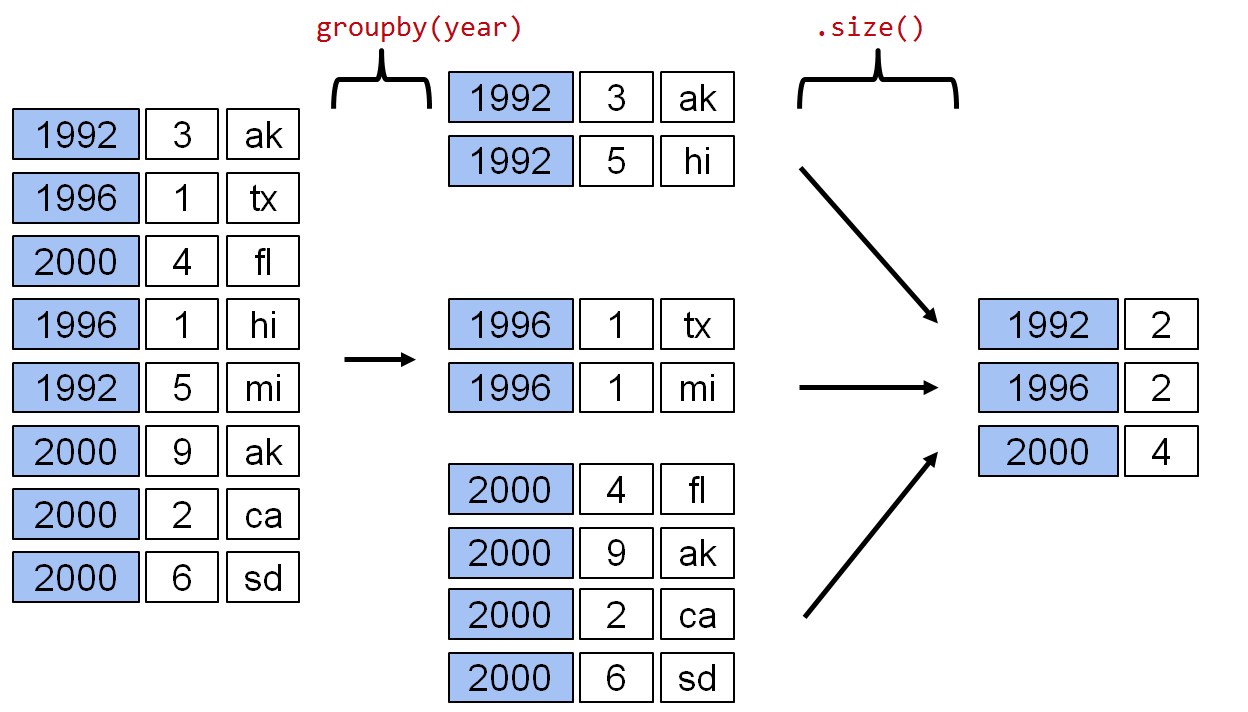
\includegraphics[scale=.33]{Bild34}
	                \end{figure}
	        \end{column}
	    \end{columns}
	 
	\end{frame}
	
	
	\begin{frame}{Overfitting and Sepal Data}
	    If we use the sepal data only (no petal data), we will run into serious overfitting issues\\
	    \bigskip
	    Below, we see our three flowers plotted in the sepal space
	    \begin{figure}
	        \centering
	        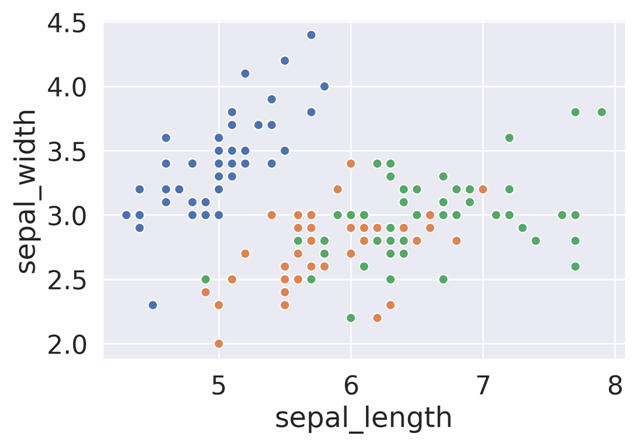
\includegraphics[scale=.65]{Bild36}
	    \end{figure}
	\end{frame}
	
	
	\begin{frame}{Sepal Decision Boundaries}
	    After training on 110/150 points, we get the decision boundaries below
	    \begin{itemize}
	        \item Decision boundaries are erratic!
	        \item Many overlapping points leads to only 93\% accuracy on training set
	    \end{itemize}
	    \begin{figure}
	        \centering
	        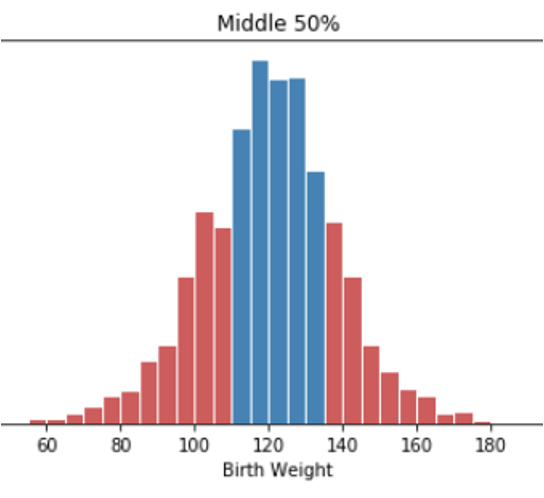
\includegraphics[scale=.65]{Bild37}
	    \end{figure}
	\end{frame}
	
	
	
	\begin{frame}{Sepal Decision Boundaries and Test Set}
	    Performance on test set is quite poor
	    \begin{itemize}
	        \item Only 70\% accuracy: 28/40 predictions are correct
	    \end{itemize}
	    \begin{figure}
	        \centering
	        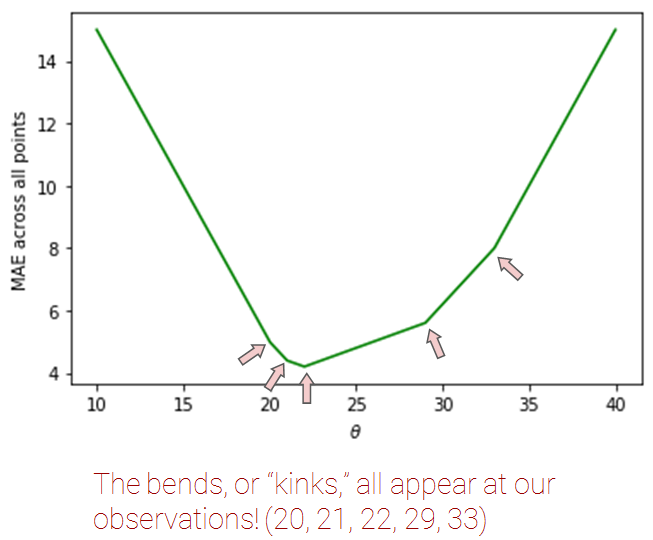
\includegraphics[scale=.65]{Bild38}
	    \end{figure}
	\end{frame}
	
	
	\begin{frame}{Overfitting Visualized}
	    The decision boundaries for our sepal model were quite complex
	    \begin{itemize}
	        \item Or drawn out as a tree, we also see a highly complex structure
	    \end{itemize}
	    Next, we’ll discuss strategies for preventing overfitting
	    \begin{figure}
	        \centering
	        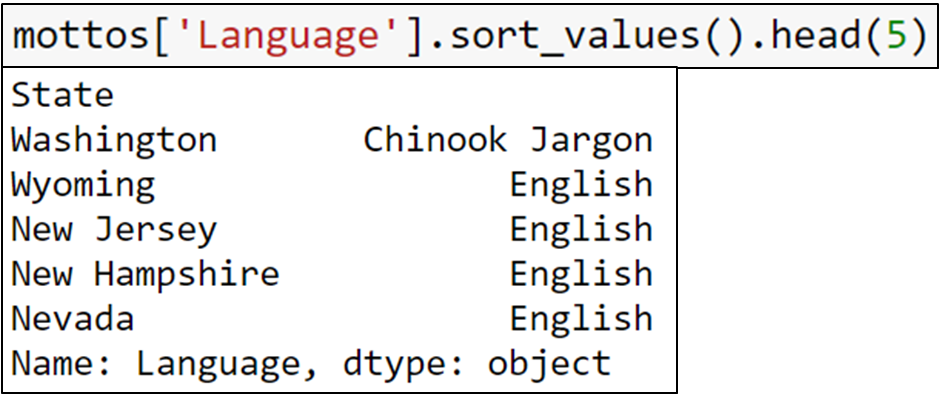
\includegraphics[scale=.5]{Bild39}
	    \end{figure}
	\end{frame}
\end{document}